\chapter{Implementación}

La implementación del software se ha dividido en hitos. Estos han sido definidos en Github (\cite{bappweb}, \cite{bappws})
y cada uno de ellos contiene un grupo de \textit{issues} que se corresponden con las distintas
mejoras que se han ido incorporando al software a lo largo de su desarrollo.\\

\section{Tecnologías}

Podemos hacer la división en Front-End y Back-End con las tecnologías utilizadas en este aplicativo. 

Para la parte de Front-End se ha utilizado una tecnología algo reciente como es ReactJS de la compañía de Facebook, aunque al ser de software libre da la posibilidad de ser mantenida por la comunidad \cite{reactjs}. React es una biblioteca de JavaScript para construir interfaces de usuario. Está siendo actualmente altamente demandada en puestos de trabajo y es una nueva forma de llevar la programación de la lógica de negocio al Front-End. Con este framework tenemos la posibilidad de construir una página web dinámica y más optimizada para el usuario, ya que React realiza una renderización por componentes y de DOM completo. 

Aunque no es requerido la sintaxis utilizada con React para la construcción del Front es JSX \cite{jsx}. Esta es una extensión de la sintaxis de JavaScript con la que podremos combinar código JavaScript con código HTML facilitando en gran medida la maquetación web y la construcción de componentes. Esto lo acompañaremos con las hojas de estilo en cascada (CSS) con las que daremos la apariencia deseada a los portales de los negocios.

En la parte de Back-End la tecnología utilizada ha sido PHP bajo el framework Symfony \cite{symfonyBook}. El uso de un framework para el Back-End es casi necesario en estos momentos, debido a que facilita el montaje de un sistema MVC si está enfocado a ello. Además, el uso de capas para la gestión de los modelos y la base de datos aumenta la seguridad del sistema como por ejemplo, evitar la inyección de código, ya que se sanitizan las entradas de datos. Otra de las ventajas que ofrece Symfony con  respecto a otros frameworks es la posibilidad de trabajar a más bajo nivel según deseemos y tener el control de cualquier proceso que implementemos en el proyecto. Sin olvidar tampoco la gran cantidad de Bundles (paquetes) desarrollados por la comunidad con funcionalidades muy interesantes como por ejemplo las sesiones con JSON Web Tokens.

\section{Librerias y Bundles}

Le sacaremos el máximo partido a las tecnologías haciendo uso de librerías y paquetes ya desarrollados con funcionalidades específicas. Vamos a destacar a continuación algunos de ellos.

\subsection{EasyAdminBundle}

Para la administración del sistema que implementaremos para el Back-End utilizaremos el Bundle EasyAdmin \cite{easyadmin} desarrollado para Symfony. Con este paquete podremos fácilmente montar una vista de administración con permisos de usuarios para la gestión completa del sistema o gestión parcial de un único negocio. Esto es posible debido a que podemos montar un Modelo-Vista-Controlador en nuestro Back-End usando como modelo las entidades ya creadas para el aplicativo. Se podrá montar el CRUD de entidades invirtiendo muy poco tiempo y esfuerzo obteniendo una vista de estas ya maquetadas.

\subsection{LexikJWTAuthenticationBundle}

Es obvio que en el sistema se deberá implementar una forma de autenticación de usuarios para poder acceder a los datos almacenados en el aplicativo. Se va a hacer uso por tanto de un Bundle desarrollado para Symfony como es LexikJWTAuthenticationBundle \cite{jwt}. Con éste tendremos la opción de manejar los inicios de sesión con JSON Web Tokens, los cuales se enviarán en las cabeceras de las peticiones de los clientes. De una forma sencilla tendremos la generación automática de estos JWT y comprobación con el usuario al cual corresponde.

\subsection{Symfony mailer}

La autenticación de usuarios será un punto necesario para los nuevos clientes que se registren en el sistema. Para ello haremos uso del Bundle Mailer y GoogleMailer para poder hacer envíos de emails, desde una cuenta de Gmail configurada para el sistema, a los usuarios recién registrados. Se implementará un servicio encargado de instanciar el mailer del Bundle y se desarrollarán funcionalidades de envío de email según las necesidades dadas. La única configuración externa al proyecto que necesitaremos será habilitar, en la cuenta de Gmail que queramos utilizar, la contraseña de 16 caracteres con la que el cliente de mail podrá acceder sin problemas.\\

Además será necesario realizar la maquetación de un email de validación junto con la lógica de negocio para no dejar al usuario iniciar sesión hasta que su cuenta haya sido verificada.

\subsection{Stripe}

En este caso haremos uso de las librerías tanto en el Front como en el Back-End debido a la dependencia de estos a la hora de realizar y gestionar los pagos. Con esta plataforma gestionaremos \textbf{intentos de pago} cuyos pasos hasta ser completados son:

\begin{itemize}
    \item \textbf{Notificación de pedido}: Para que un intento de pago pueda darse, primero, un cliente deberá acceder a su carrito de la compra (no vacío), seleccionar una de sus direcciones postales y pulsar en el botón de continuar. Una vez hecho esto se realizará una llamada al Web Service, creando un pedido en el sistema con estado pendiente.
    \item \textbf{Creación de intento de pago}: Si el pedido se ha creado correctamente, se procederá a crear inmediatamente un intento de pago haciendo uso del \textbf{StripeClient} proporcionado por el Bundle. Si no ha ocurrido ningún error, se generarán dos valores: el ID del intento de pago en Stripe y el ClientSecret necesario para realizar el pago en la parte de Front. Estos valores se establecerán en el pedido creado y se devolverá como respuesta de Web Service al usuario.
    \item \textbf{Pago}: Una vez recibido el pedido cargaremos el formulario donde se introducirá la tarjeta de crédito. Tras completar los datos, podremos confirmar el pago junto con el ClientSecret establecido en el pedido haciendo uso de un hook de Stripe. Si no ha ocurrido ningún error en el pago, se notificará de nuevo al Web Service que ese pedido ha sido pagado con éxito para cambiar su estado en base de datos.
\end{itemize}

\begin{figure}[H]
  \centering
  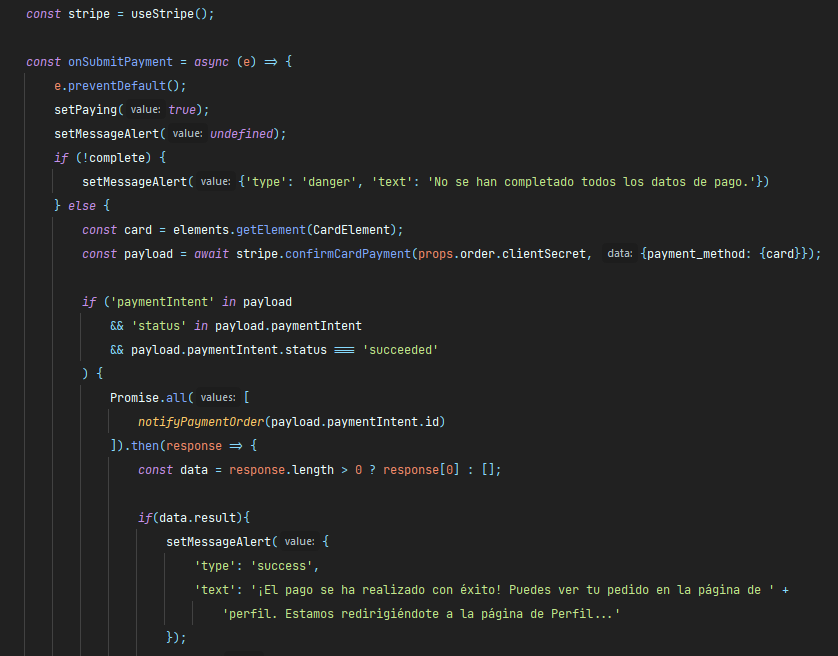
\includegraphics[scale=0.5]{images/front-end-stripe.png}
  \caption{Confirmación de pago en ReactJS con Stripe}
  \label{}
\end{figure}

\begin{figure}[H]
  \centering
  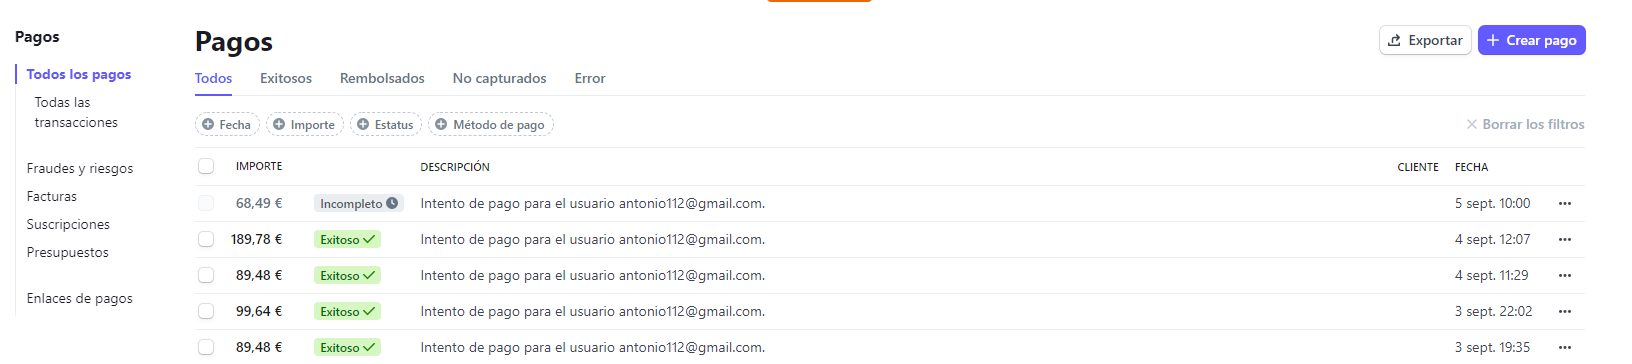
\includegraphics[scale=0.25]{images/back-end-stripe.png}
  \caption{Historial de pagos en la plataforma Stripe}
  \label{}
\end{figure}

\subsection{Axios} 

Realizaremos las llamadas al Back-End desde la parte del cliente con Axios \cite{axios}. Con esta librería podremos hacer llamadas asíncronas a los datos de nuestro sistema para eliminar los tiempos de carga completos de nuestras páginas webs. Esto es una parte importante del planteamiento de Front, ya que el objetivo es hacer páginas dinámicas donde el usuario no se vea imposibilitado de interactuar con la web mientras espera la renderización de los productos de la tienda por ejemplo. También las llamadas asíncronas mejorarán la velocidad de carga de estas gracias al DOM se irá cargando poco a poco de manera asíncrona y no estará en su mayor parte bloqueado por la renderización completa. 

\subsection{Reporte de errores con Telegram} 

Todo sistema informático está expuesto a posibles errores no esperados por los desarrolladores. Detectar estos problemas a tiempo puede ser fundamental para el correcto funcionamiento del aplicativo o la defensa ante posibles patrones de ataques.
Para ello usaremos la API de TelegramBot \cite{telegrambot} con la que podremos enviarnos notificaciones desde el servidor hasta un Bot de Télegram previamente configurado.\\
Podremos hacer uso del servicio \textbf{TelegramService}:

\begin{figure}[H]
  \centering
  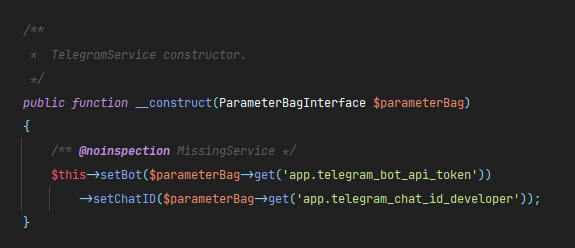
\includegraphics[scale=0.8]{images/telegram-service-0.png}
  \caption{Constructor de TelegramService: inicialización de parámetros}
  \label{}
\end{figure}

\begin{figure}[H]
  \centering
  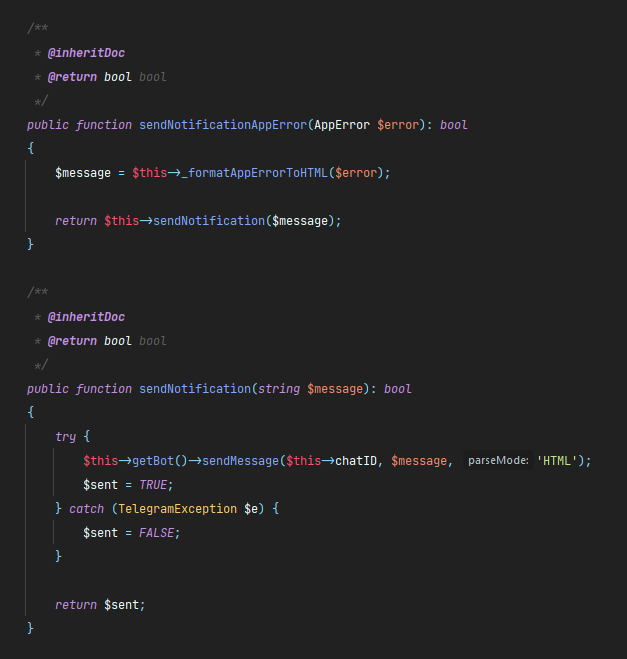
\includegraphics[scale=0.8]{images/telegram-service-1.png}
  \caption{Métodos públicos de TelegramService: enviar mensajes y AppErrors}
  \label{}
\end{figure}

\begin{figure}[H]
  \centering
  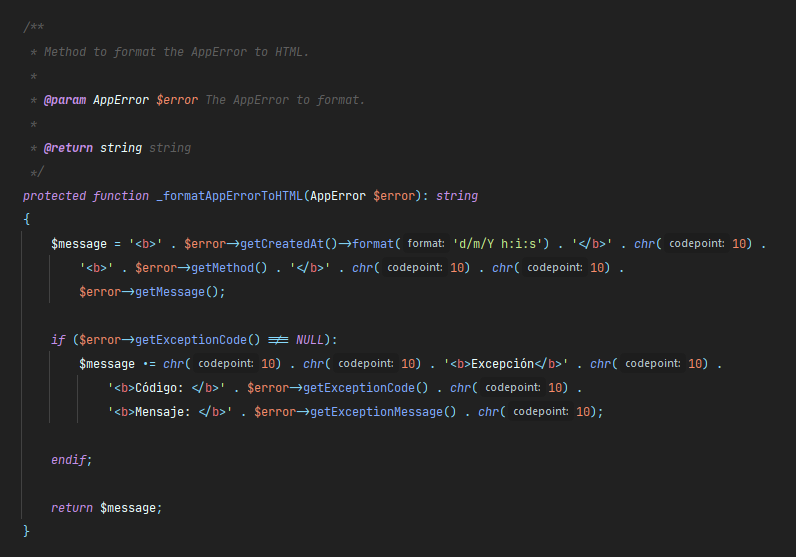
\includegraphics[scale=0.5]{images/telegram-service-2.png}
  \caption{Método privado de TelegramService: formatear mensaje de error}
  \label{}
\end{figure}

\section{Estructuración de código en Symfony}

En este proyecto Symfony vamos a tener los siguientes tipos de archivos:

\begin{itemize}
    \item \textbf{Controller}: Los controladores serán los encargados de recibir las peticiones realizadas al servidor y sanitizar y validar los datos recibidos por el Request.
    \item \textbf{Entity}: Las entidades serán nuestro modelo de datos. Dentro de las entidades haremos uso de una herramienta denominada Annotations de Doctrine. Con esto definiremos nuestras tablas, atributos, relaciones y restricciones de la base de datos del Sistema.
    \item \textbf{Traits}: Los trait son trozos de código los cuales podremos inyectar en nuestros diferentes ficheros según necesitemos. Principalmente los usaremos para definir propiedades comunes de entidades y así evitar la duplicidad de código en el proyecto.
    \item \textbf{Repository}: Los repositorios serán los encargados de recuperar las entidades de datos que tengamos almacenados. Con estos se podrán hacer consultas a la base de datos sin necesidad de realizar sentencias SQL directamente.
    \item \textbf{Service}: Los servicios serán la capa bajo los controladores. Estos se encargarán de realizar la lógica de negocio correspondiente a cada petición de los usuarios. Será la única capa con acceso a los repositorios de las entidades en la que se podrán persistir objetos ORM.
    \item \textbf{Interfaces}: Habrá interfaces por cada archivo del proyecto para tener una documentación completa de todas las funcionalidades implementadas.
    \item \textbf{Helpers}: Los helpers serán archivos con funcionalidades de ayuda como su nombre indica. Funcionalidad fuera de la lógica de negocio que nos puede facilitar cálculos repetitivos.
\end{itemize}

Con esta estructura podríamos decir que nuestro flujo sería el siguiente: el cliente realiza una petición al servidor. Esta llega a la ruta definida en uno de los controladores donde se tratarán los datos obtenidos del Request de manera que si no son válidos, reporte el correspondiente error al cliente. En el caso de ser válidos pasarán al respectivo Servicio (normalmente un controlador deberá tener inyectado un servicio). En él se ejecutará la lógica de negocio definida donde se creará, recuperará, modificará o eliminará una entidad definida. Una vez procesado se devolverán los datos correspondientes al controlador (ya sean errores o los datos solicitados) y el controlador los devolverá al cliente con una respuesta en formato JSON.

\begin{figure}[H]
  \centering
  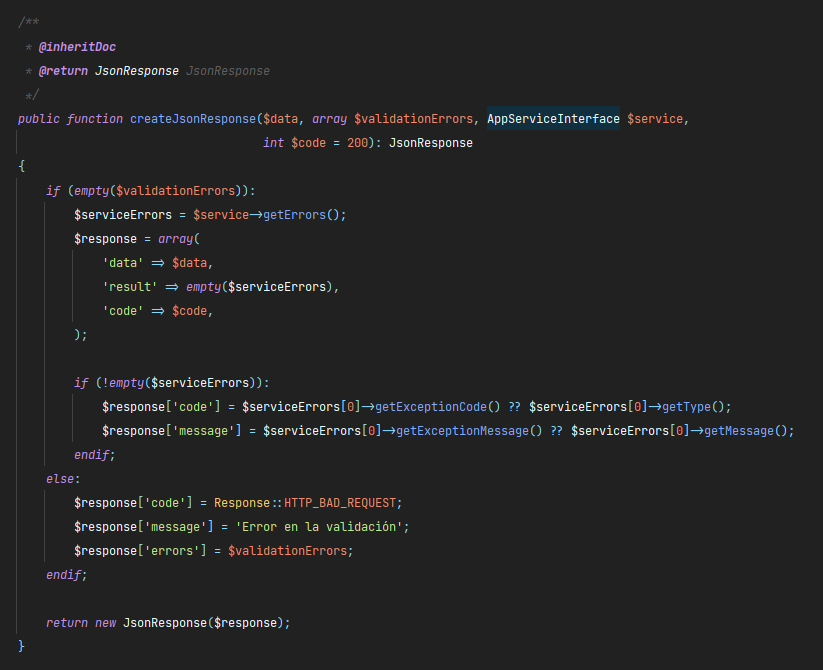
\includegraphics[scale=0.5]{images/create-json-response.png}
  \caption{Funcionalidad de AppController: creación de respuesta JSON para API}
  \label{}
\end{figure}

Todo esto proceso registrará, en caso de producirse, errores en el aplicativo que serán notificados por Telegram como bien hemos comentado en un apartado anterior. Gracias a estas notificaciones y registro de errores el control para el superadministrador del aplicativo será mucho mayor pudiendo solucionar errores en un menor periodo de tiempo.


\section{Estructuración de código en ReactJS}

El objetivo de usar ReactJS es el trabajar con componentes con los que facilitarnos la maquetación y el control de los estados de la aplicación. Para ello vamos a estructurar nuestro código de la siguiente manera:

\begin{itemize}
    \item \textbf{App.js}: Será el archivo principal de la aplicación donde definiremos el routing. Además añadiremos los componentes comunes como pueden ser el Header y el Footer que no recibirán modificaciones en las diferentes vistas.
    \item \textbf{Services}: Aquí almacenaremos los diferentes servicios de nuestra aplicación. Estos serán los encargados de intercambiar información con el Web Service. Separando la lógica de comunicación de lo que son los componentes ganamos en abstracción, ya que, si en algún momento recuperamos los datos de un sitio solamente deberemos actualizar el servicio sin que nada afecte al funcionamiento de la aplicación.
    \item \textbf{Components}: Tendremos un directorio con componentes comunes. El encapsulamiento de estos nos ahorrará trabajo a la hora del diseño Web con lo que conseguiremos no repetir código y tener una mayor homogeneidad a los ojos del usuario.
    \item \textbf{Directorios de páginas}: Por último tendremos nuestros directorios referentes a cada página del proyecto así como los distintos componentes de los que se compone.
\end{itemize}

\section{Uso y funcionamiento}

En esta sección vamos a repasar el funcionamiento de la herramienta, a nivel de Front-End y Back-End, y ver en como afecta la configuración registrada en la administración a la aplicación Web.

\subsection{Página de Home}

Como bien se ha explicado, la página de Home se ha hecho de una forma configurable para los trabajadores del negocio, pudiendo mostrar así la información que deseen. Vamos a ver a continuación las comparativas de configuración en la administración y la visualización en la Web:

\subsection{Sección de Introducción}

\begin{figure}[H]
  \centering
  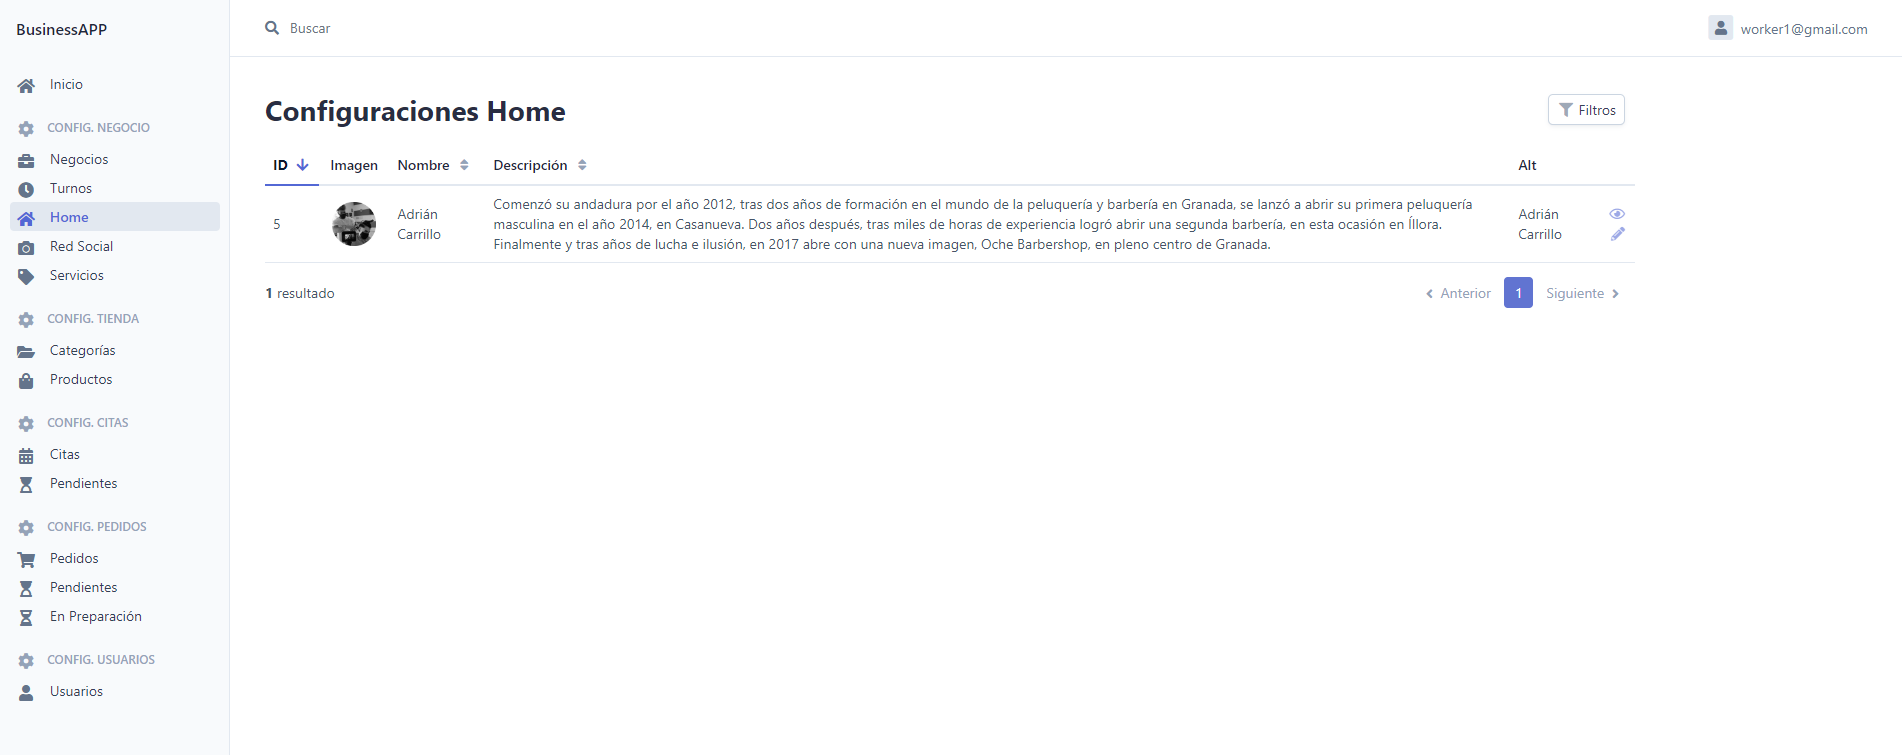
\includegraphics[scale=0.2]{images/back-end-introduction.png}
  \caption{Configuración de la sección de Introducción en el Back-End}
  \label{}
\end{figure}

\begin{figure}[H]
  \centering
  
\includegraphics[scale=0.2]{images/front-end-introduction.png}
  \caption{Renderización de la configuración en la Web}
  \label{}
\end{figure}

\subsection{Sección de Red Social}

\begin{figure}[H]
  \centering
  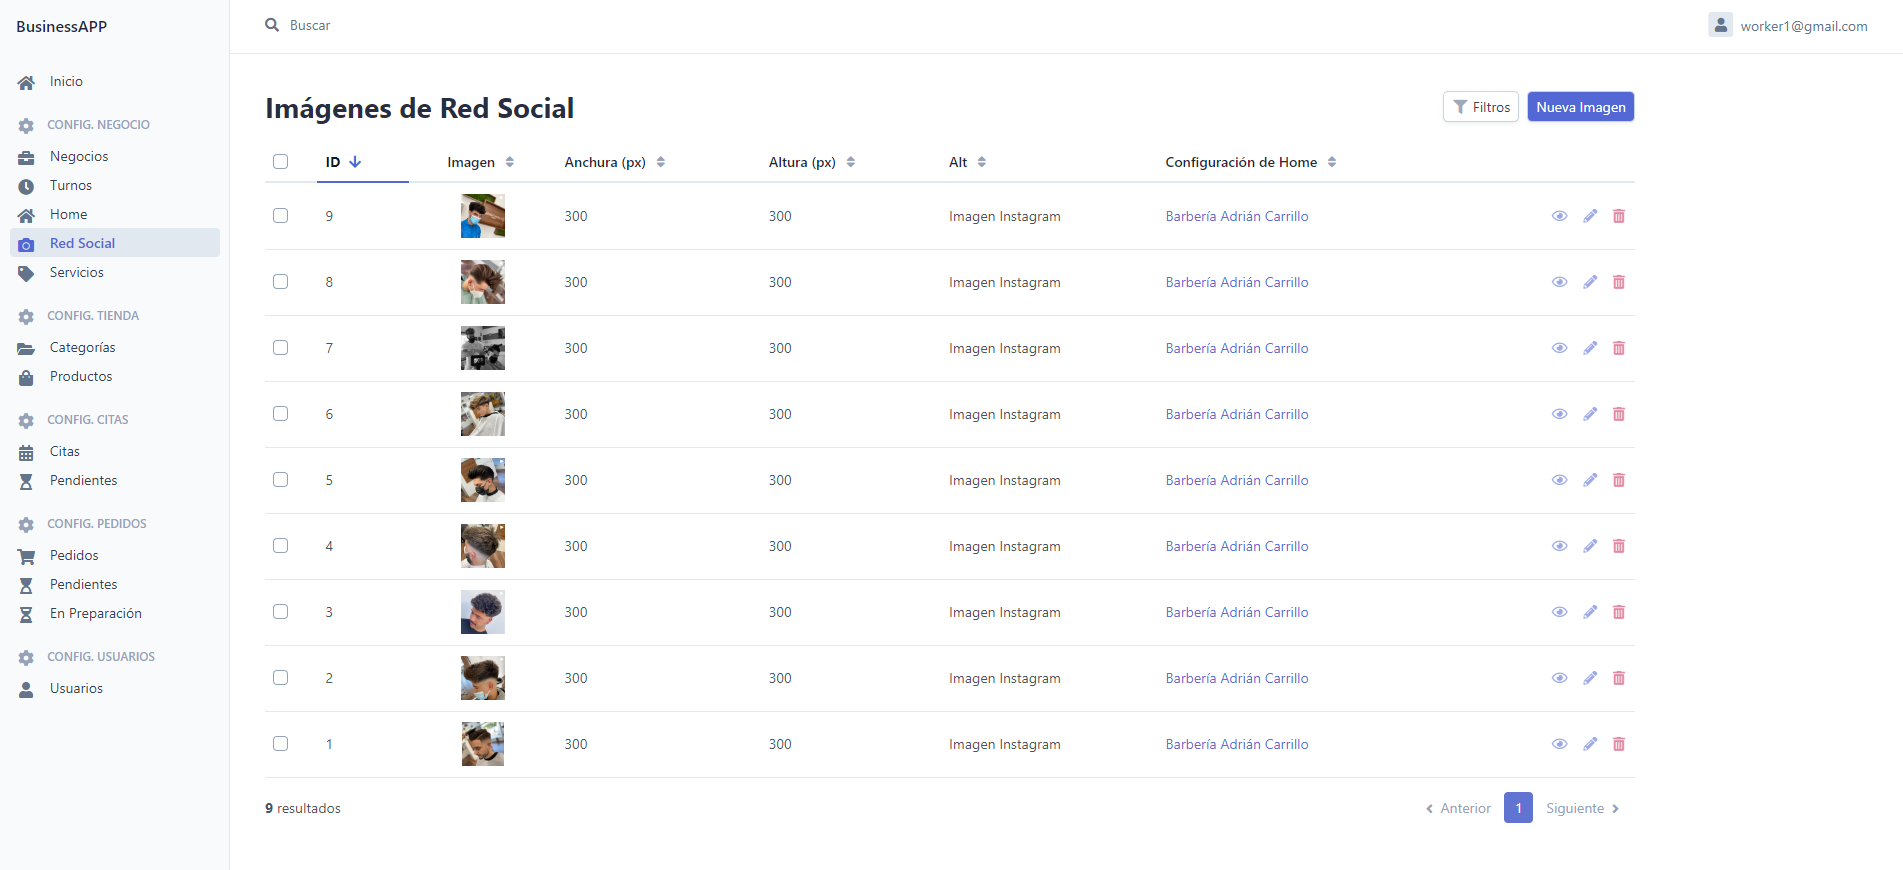
\includegraphics[scale=0.2]{images/back-end-social.png}
  \caption{Configuración de la sección de Red Social en el Back-End}
  \label{}
\end{figure}

\begin{figure}[H]
  \centering
  
\includegraphics[scale=0.2]{images/front-end-social.png}
  \caption{Renderización de la configuración en la Web}
  \label{}
\end{figure}

\subsection{Sección de Servicios}

\begin{figure}[H]
  \centering
  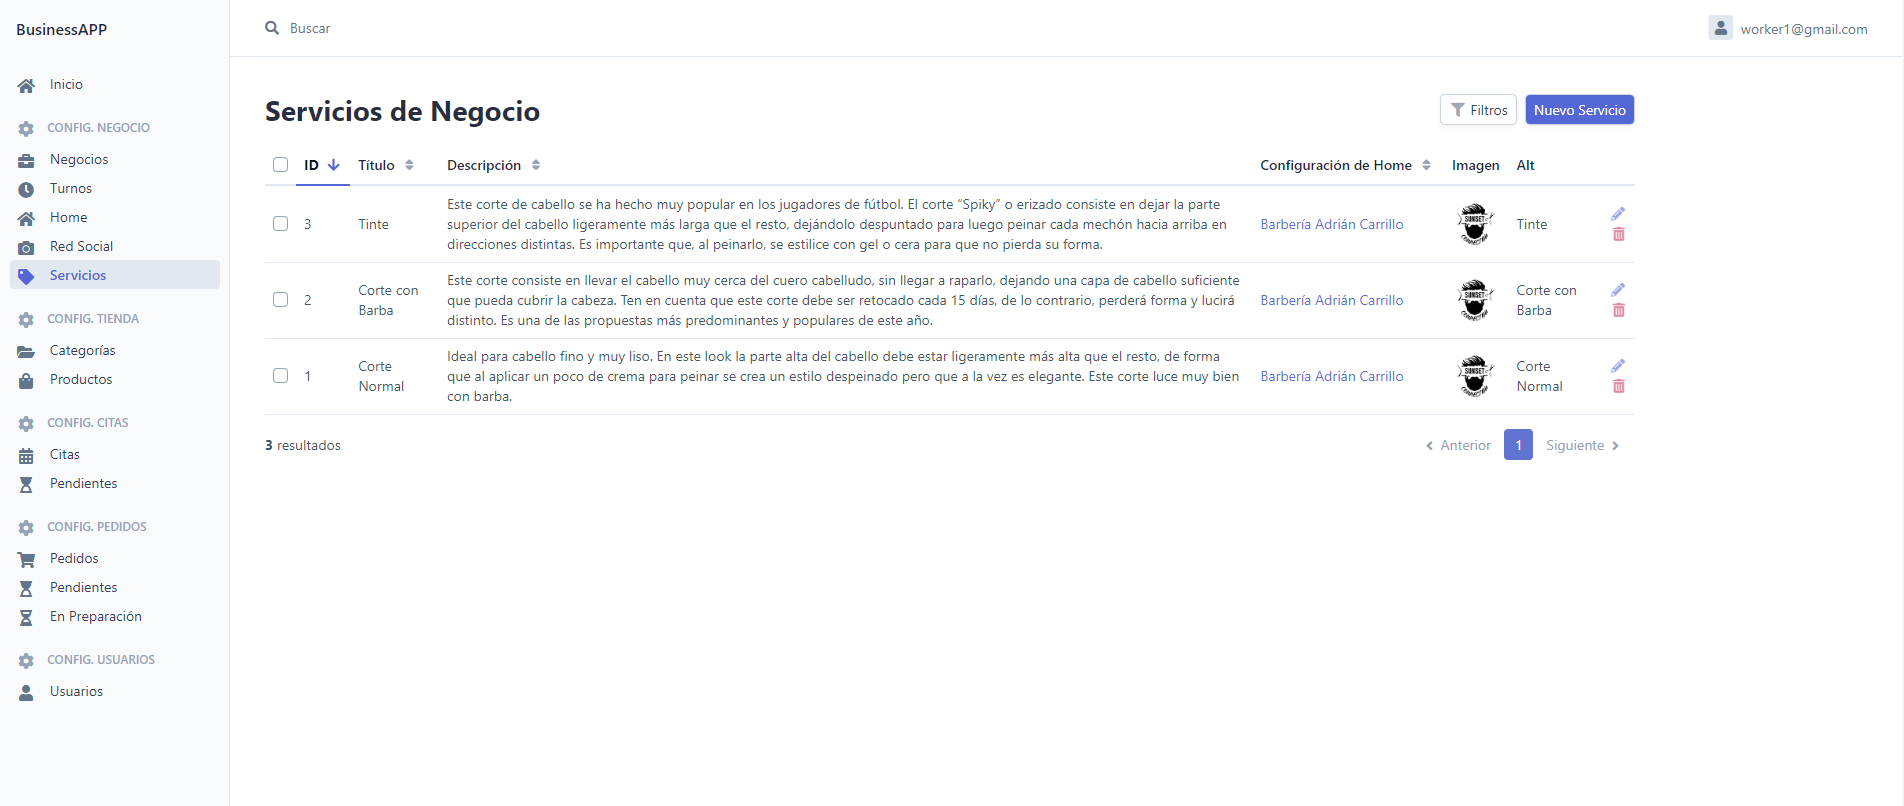
\includegraphics[scale=0.2]{images/back-end-services.png}
  \caption{Configuración de la sección de Servicios ofrecidos en el Back-End}
  \label{}
\end{figure}

\begin{figure}[H]
  \centering
  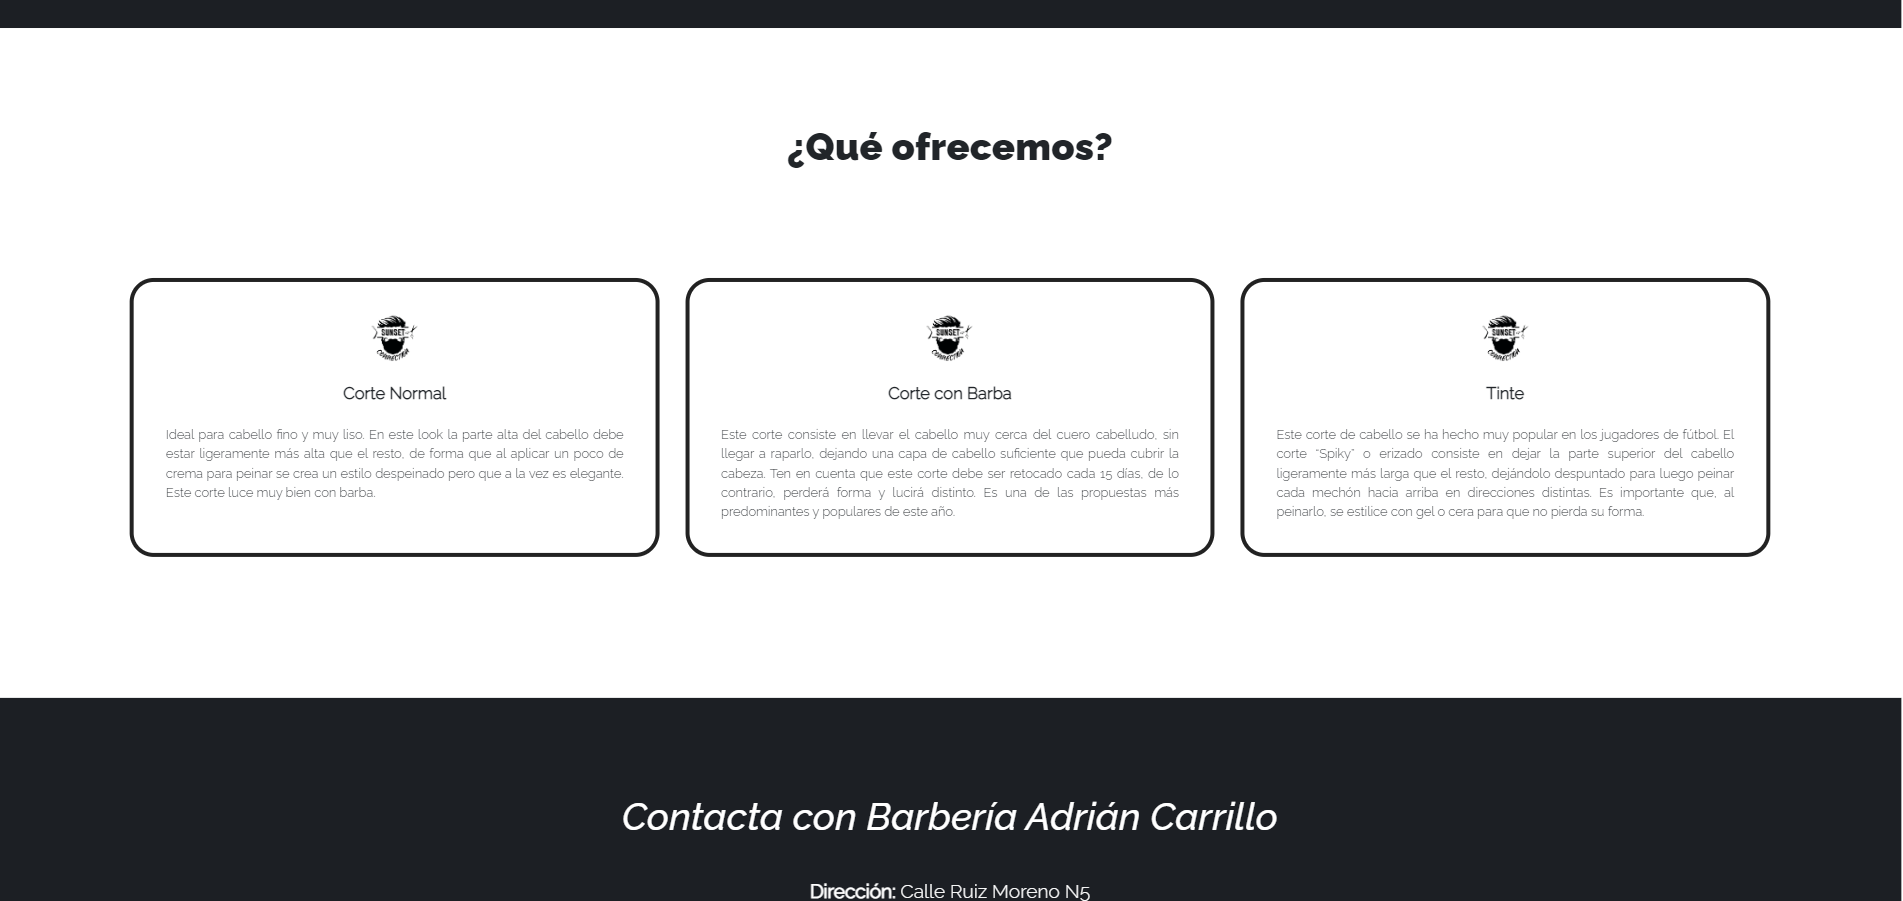
\includegraphics[scale=0.2]{images/front-end-services.png}
  \caption{Renderización de la configuración en la Web}
  \label{}
\end{figure}

\subsection{Sección de Información del negocio}

\begin{figure}[H]
  \centering
  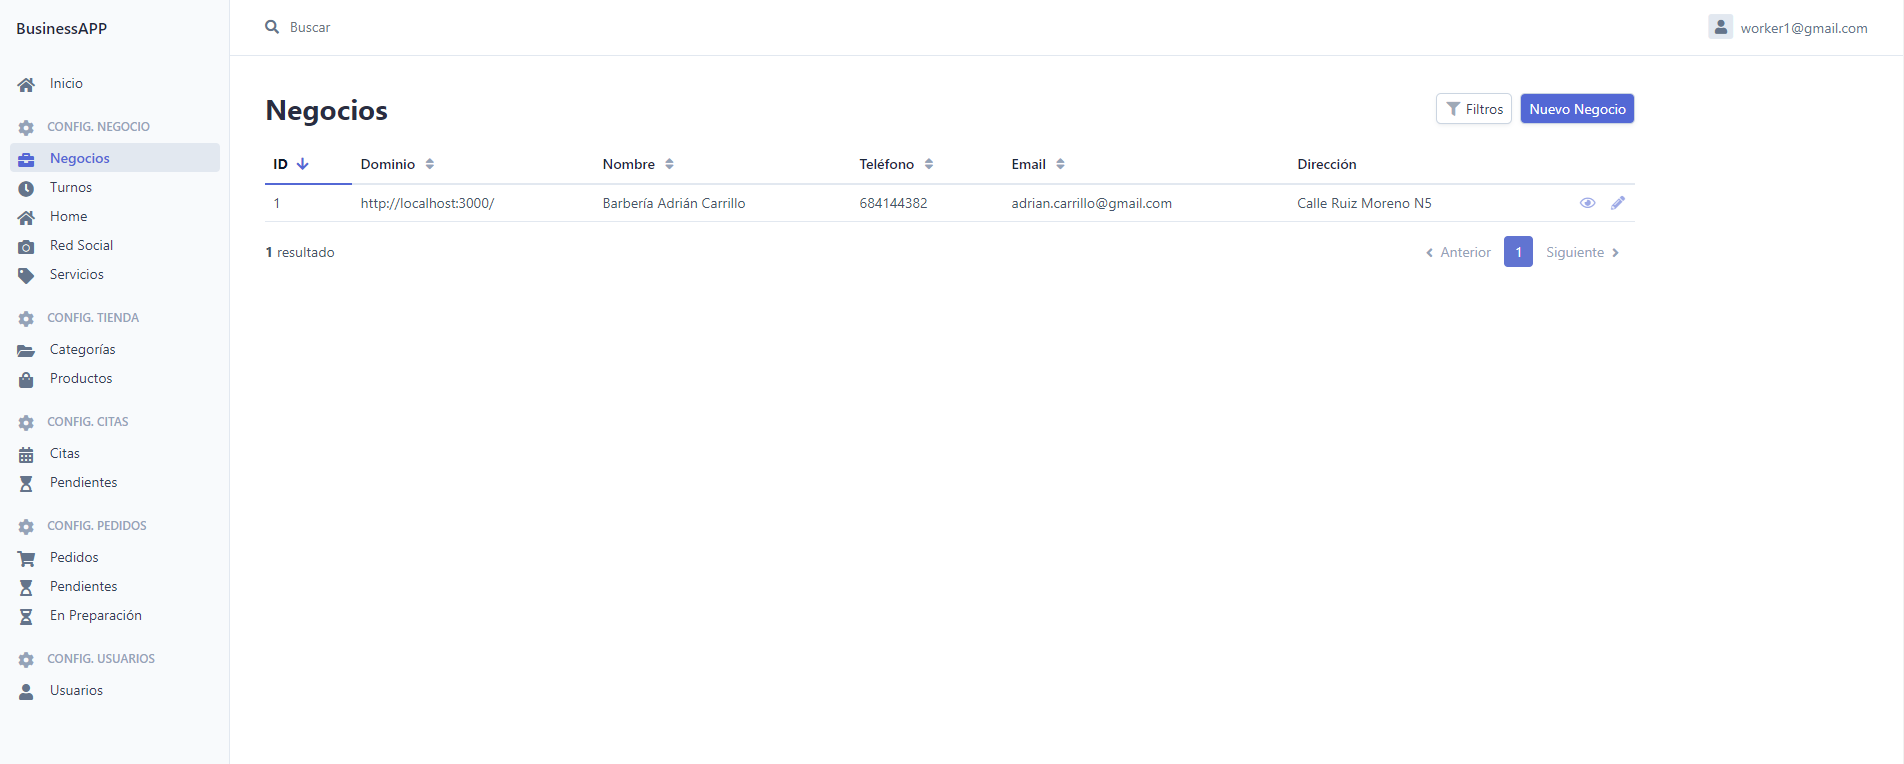
\includegraphics[scale=0.2]{images/back-end-info-business.png}
  \caption{Configuración de la sección de Información del negocio en el Back-End}
  \label{}
\end{figure}

\begin{figure}[H]
  \centering
  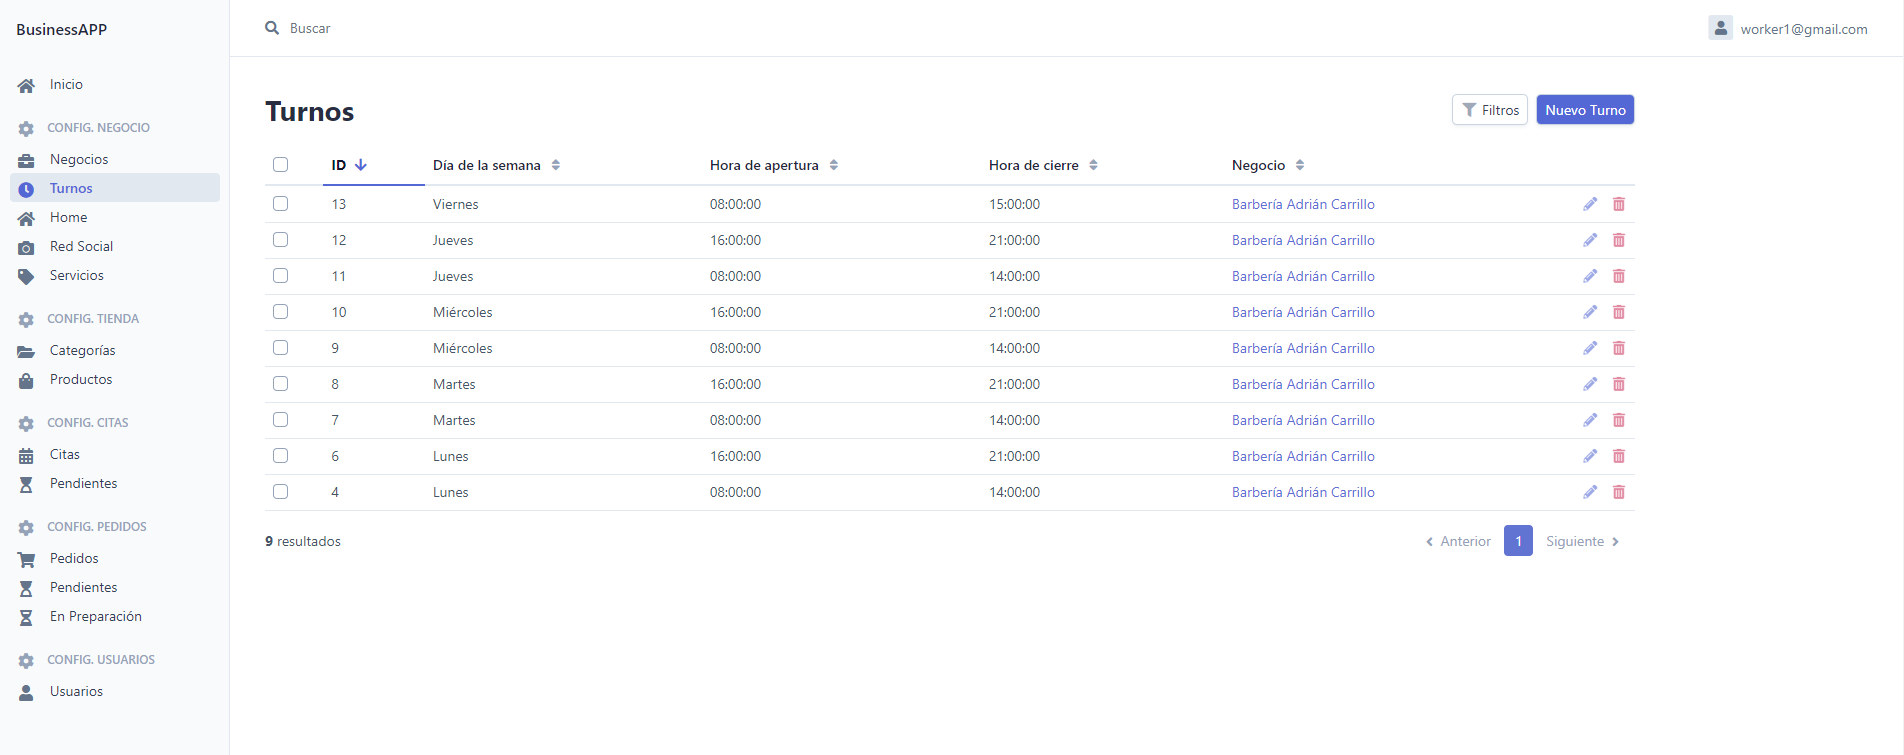
\includegraphics[scale=0.2]{images/back-end-shifts.png}
  \caption{Configuración de los turnos del negocio en el Back-End}
  \label{}
\end{figure}

\begin{figure}[H]
  \centering
  
\includegraphics[scale=0.2]{images/front-end-shifts.png}
  \caption{Renderización de la configuración en la Web}
  \label{}
\end{figure}

\subsection{Página de Productos}

En la página de productos también estará la posibilidad de crear, editar o eliminar lo ofertado, pudiendo crear también a su vez las categorías de estos para realizar filtros en la Web. A continuación veremos las comparativas de esta sección:

\begin{figure}[H]
  \centering
  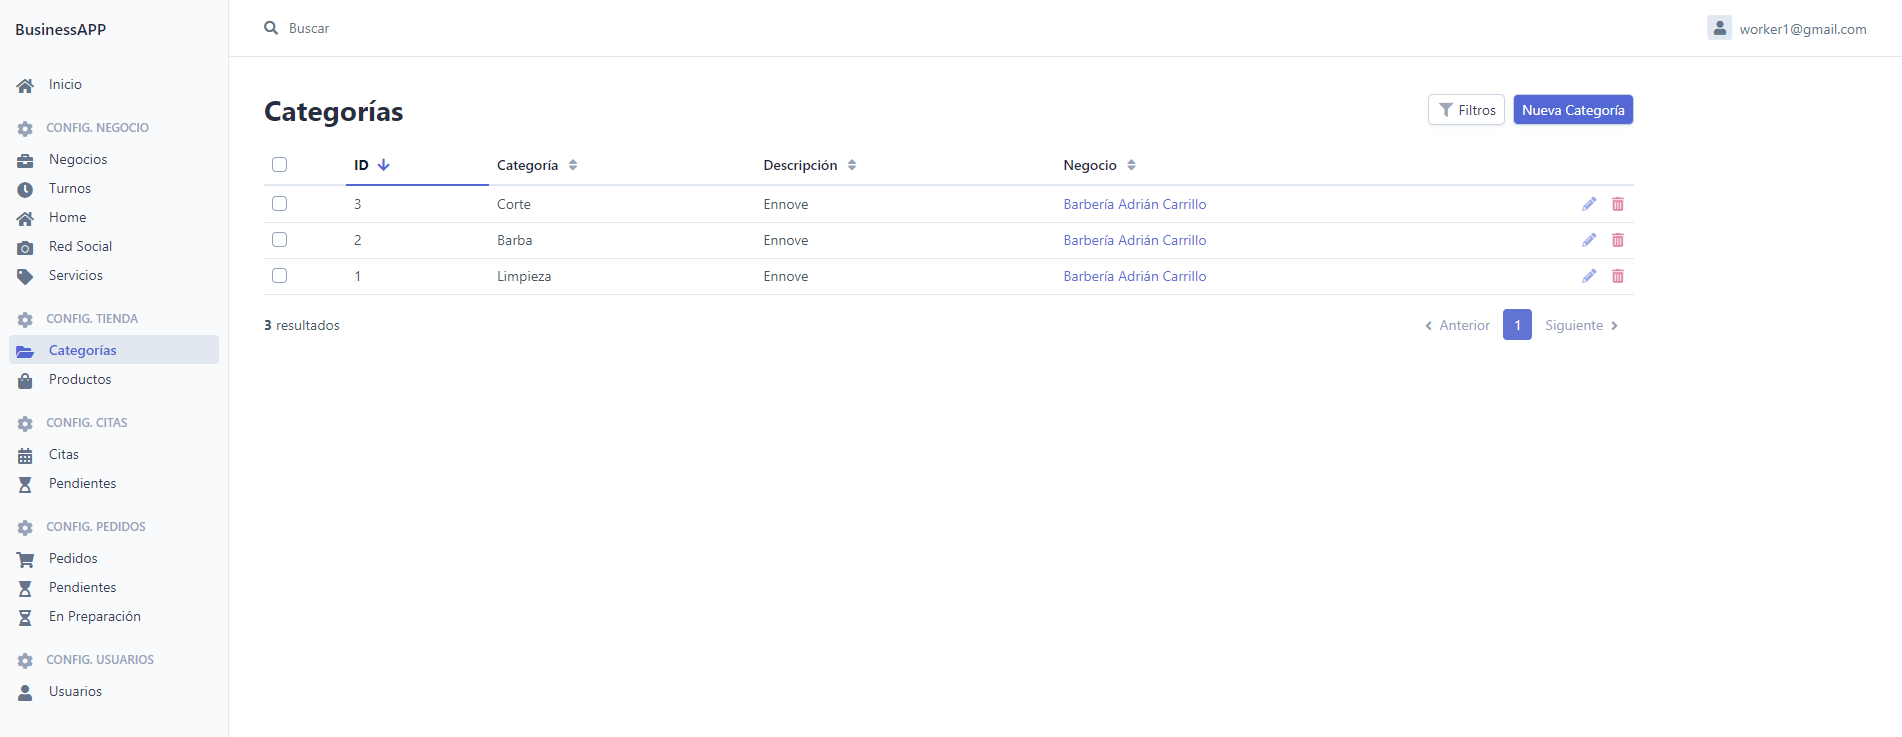
\includegraphics[scale=0.2]{images/back-end-categories.png}
  \caption{Configuración de las categorías de productos del negocio en el Back-End}
  \label{}
\end{figure}

\begin{figure}[H]
  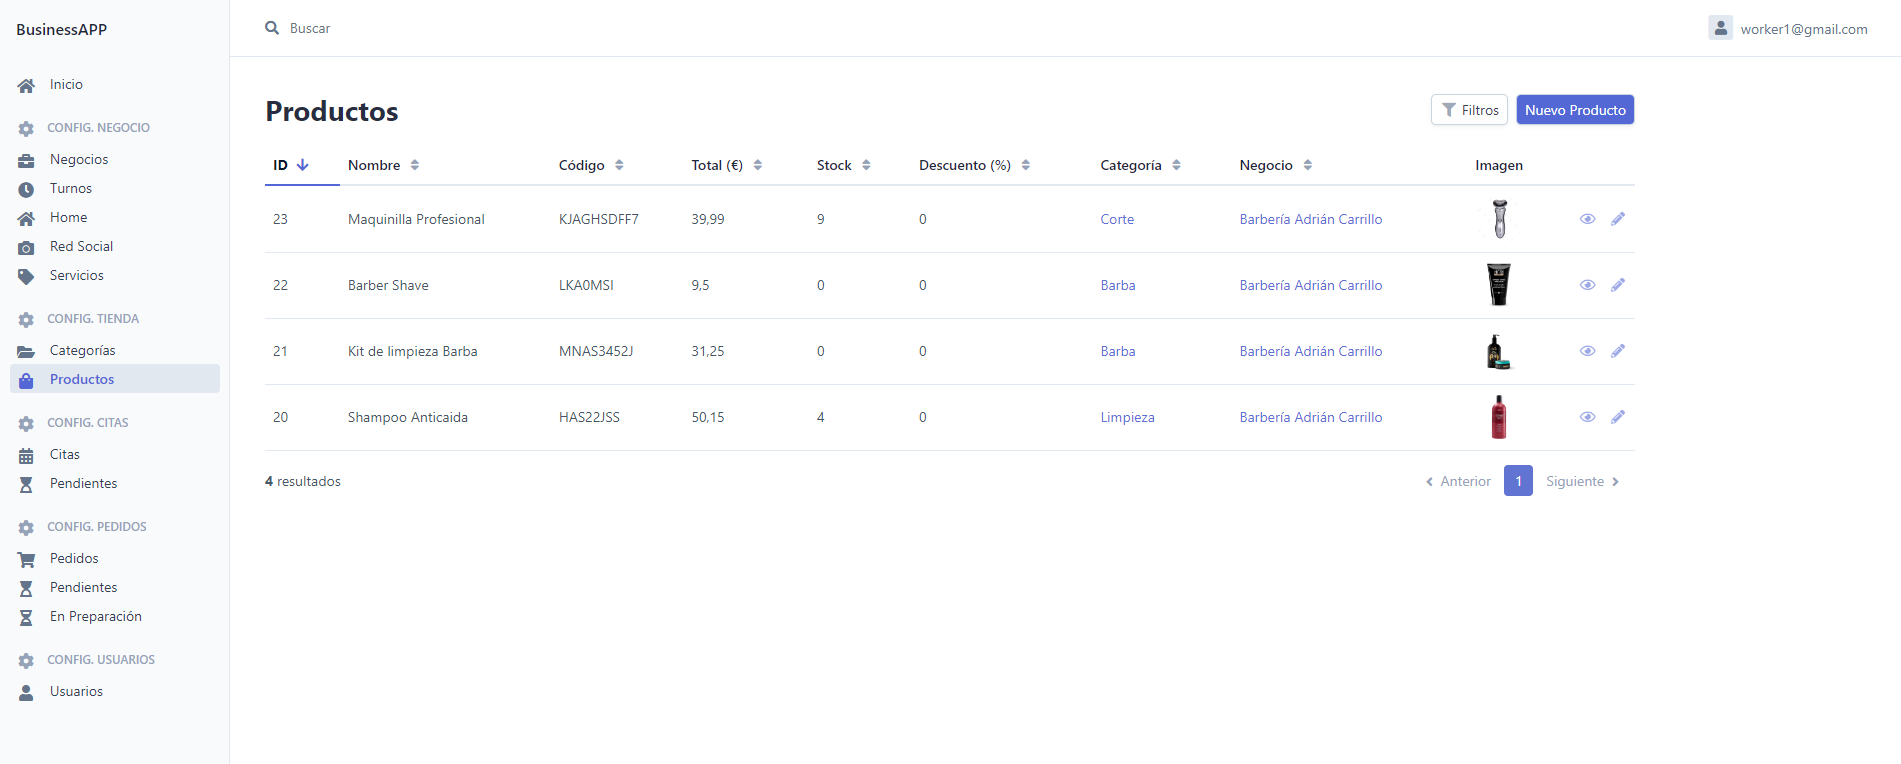
\includegraphics[scale=0.2]{images/back-end-products.png}
  \caption{Configuración de los productos vendidos por el negocio en el Back-End}
  \label{}
\end{figure}

\begin{figure}[H]
  \centering
  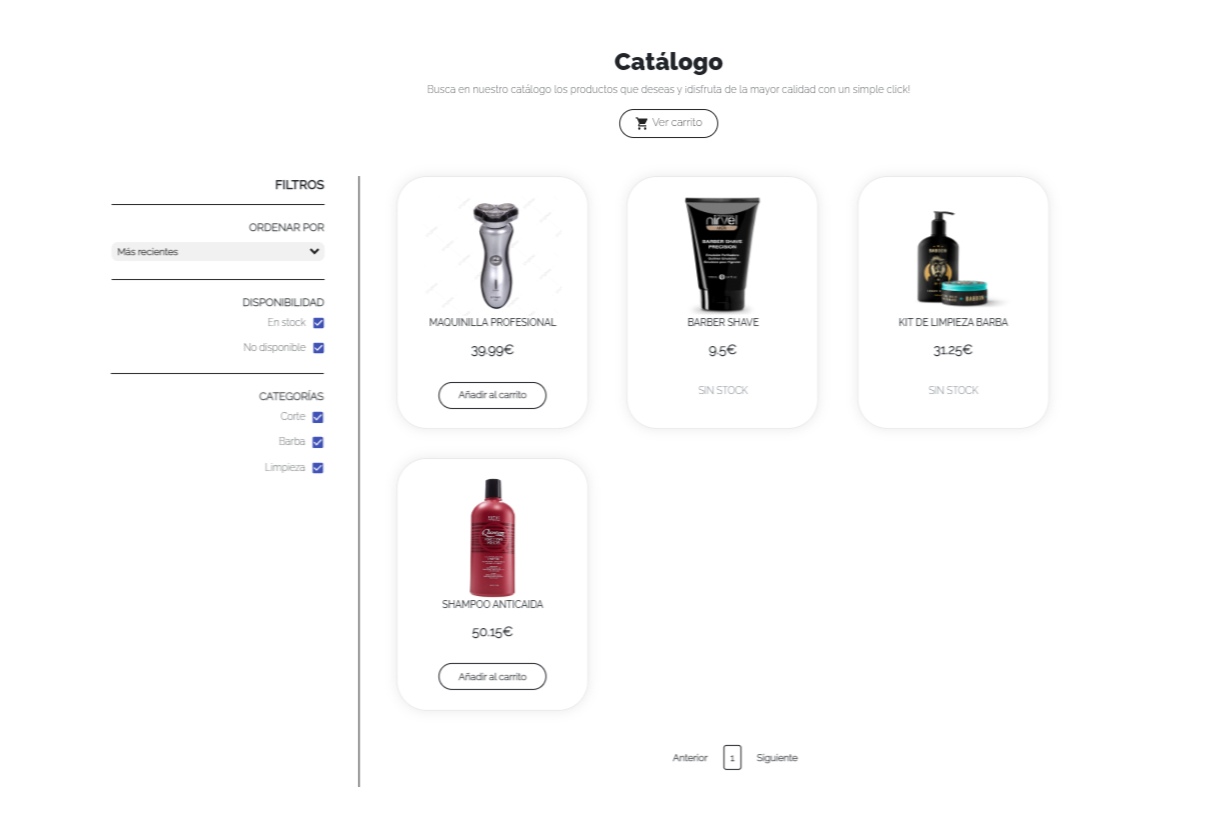
\includegraphics[scale=0.3]{images/front-end-products.png}
  \caption{Renderización de la configuración en la Web}
  \label{}
\end{figure}

\begin{figure}[H]
  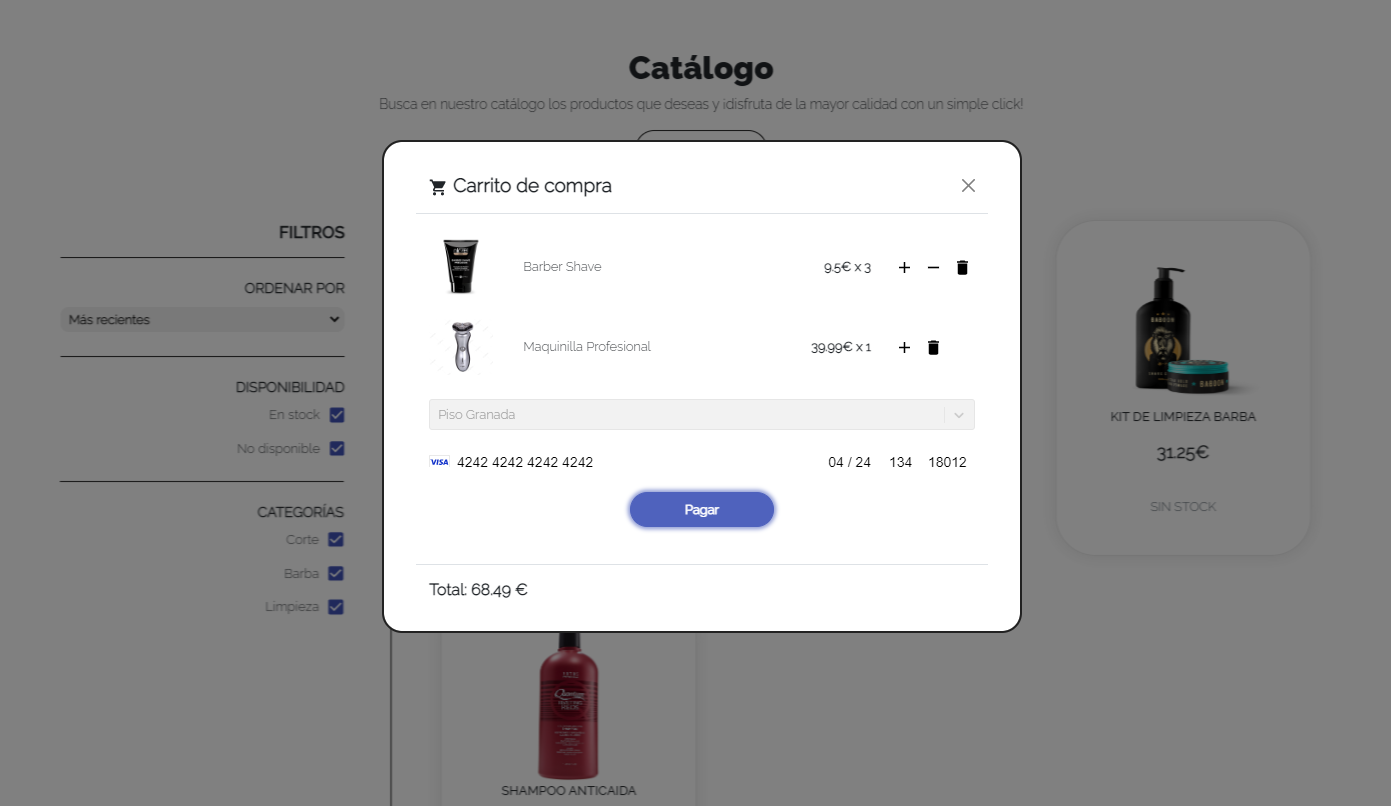
\includegraphics[scale=0.35]{images/front-end-payment.png}
  \caption{Carrito de compra en proceso de pago}
  \label{}
\end{figure}

\subsection{Página de Citas}

La página de citas usará la información de configuración de turnos del negocio para la renderización del número de citas por día. Además consultará al Web Service las citas ya reservadas en un día seleccionado para habilitar o deshabilitar en la página Web aquellas horas que estén o no disponibles.\\
Si un usuario tiene una reserva activa no podrá realizar otra reserva hasta completarse o cancelarse la actual. Se informará con una alerta en los días seleccionados.

\begin{figure}[H]
  \centering
  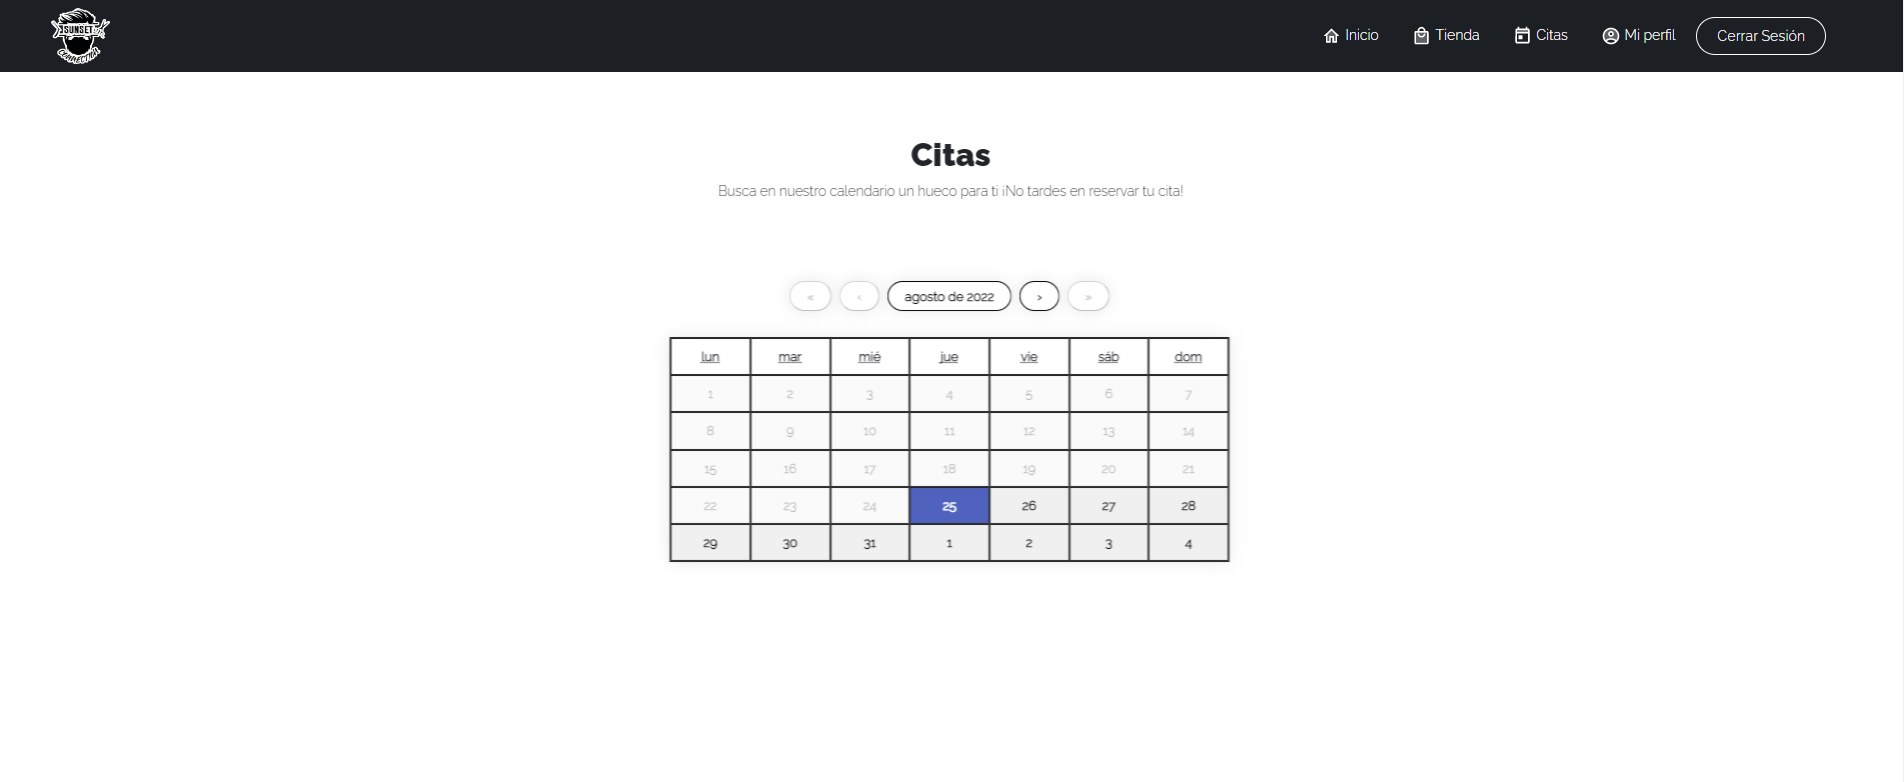
\includegraphics[scale=0.2]{images/front-end-appointment-1.png}
  \caption{Página de citas: vista inicial}
  \label{}
\end{figure}

\begin{figure}[H]
  \centering
  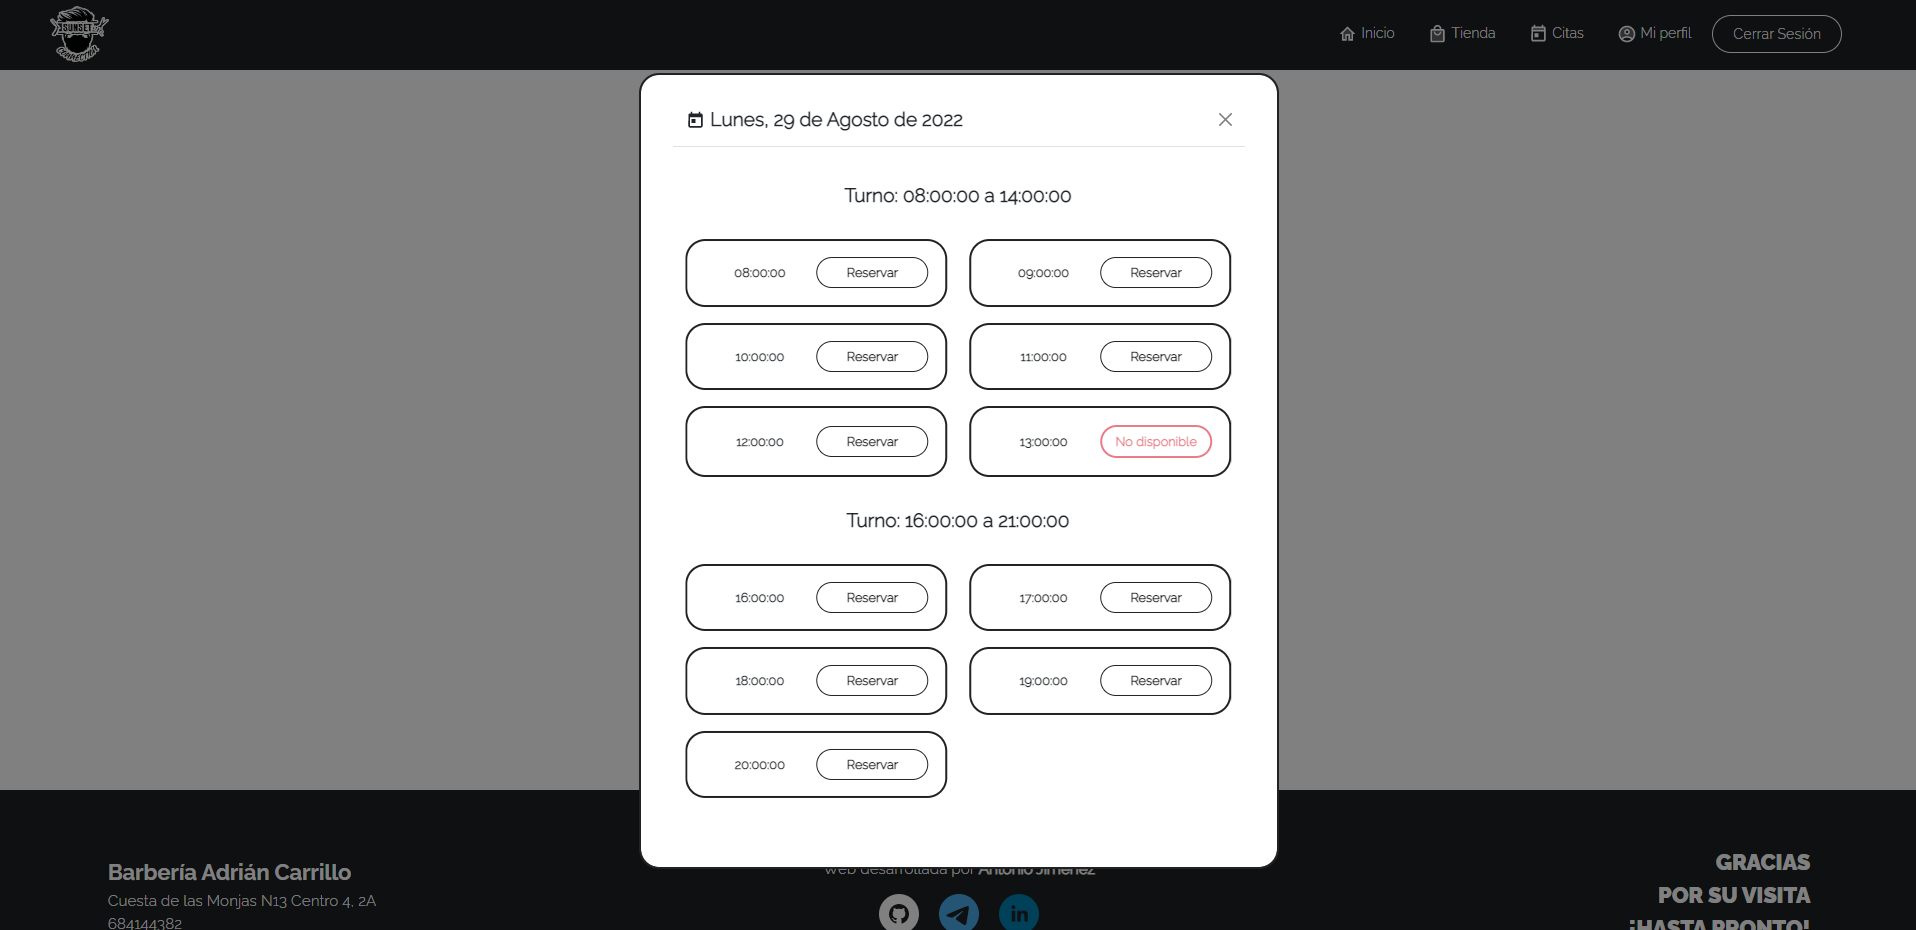
\includegraphics[scale=0.2]{images/front-end-appointment-2.png}
  \caption{Página de citas: día seleccionado}
  \label{}
\end{figure}

\begin{figure}[H]
  \centering
  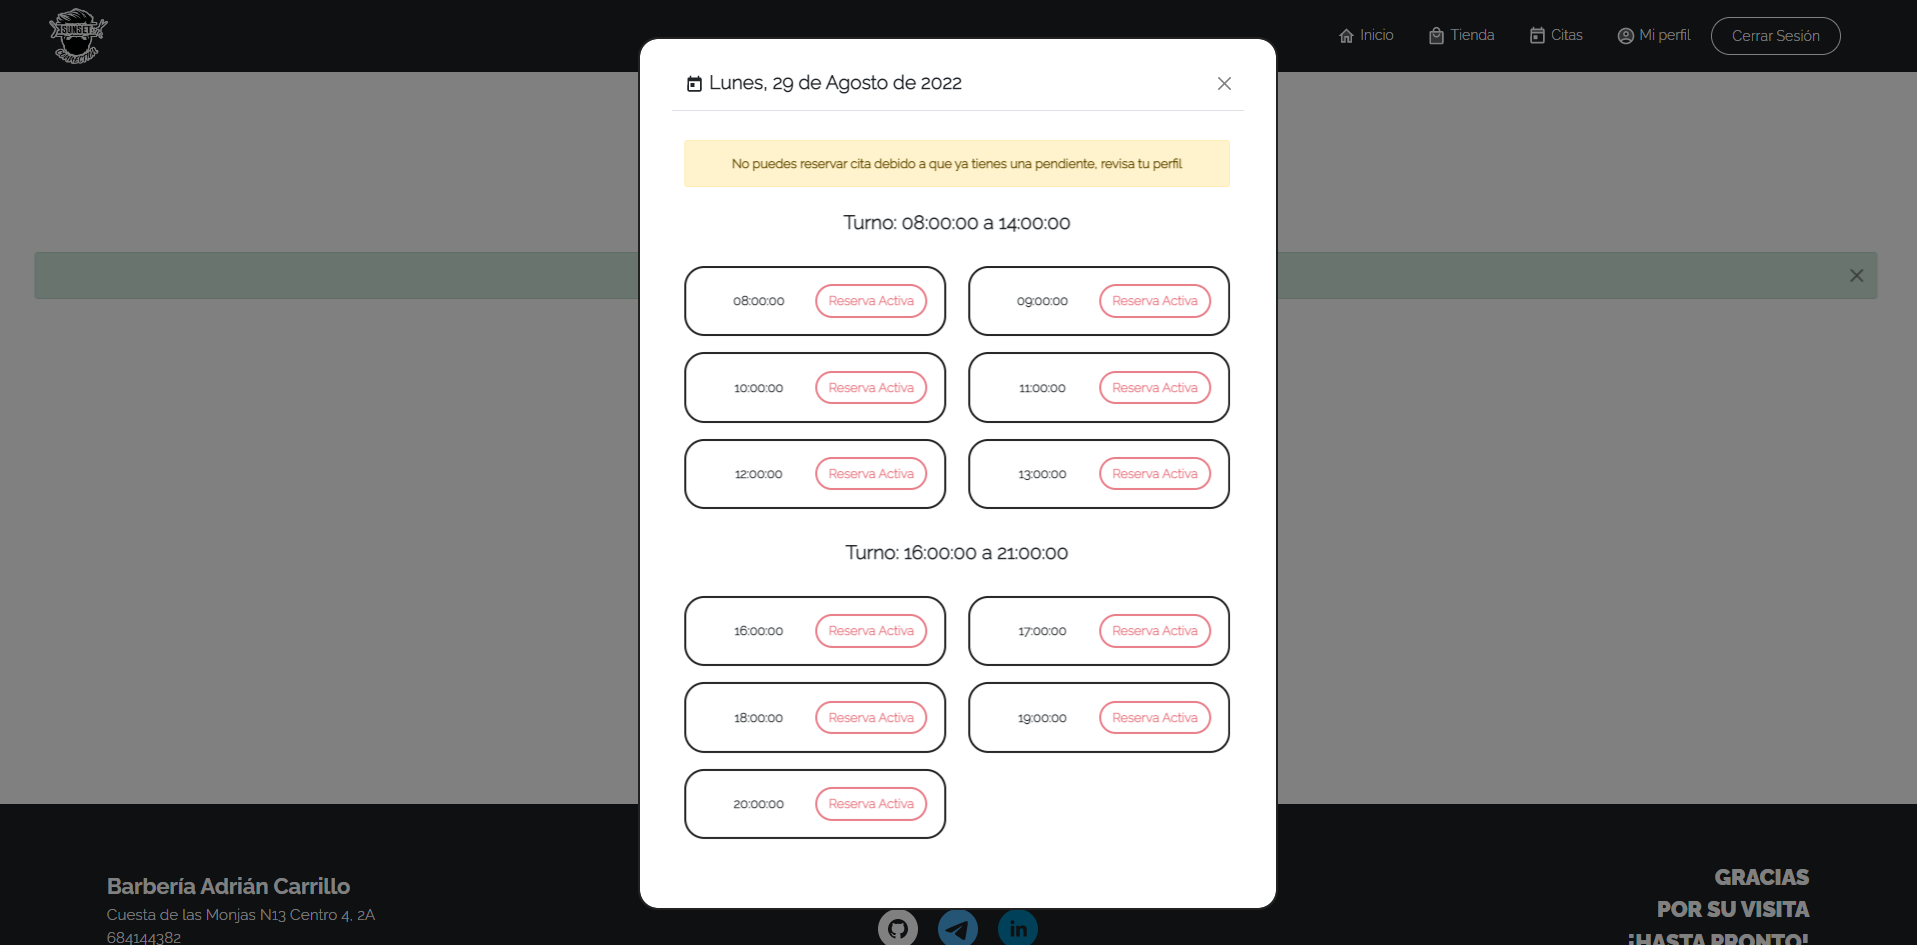
\includegraphics[scale=0.2]{images/front-end-appointment-3.png}
  \caption{Página de citas: usuario con cita pendiente}
  \label{}
\end{figure}

\subsection{Página de Perfil}

Por último tenemos la página de Perfil. En esta el usuario tendrá la posibilidad de editar sus datos personales; crear, editar o eliminar sus direcciones postales (que deberá usar para realizar pedidos online); y ver sus historiales de pedidos y citas así como realizar las cancelaciones pertinentes.

\begin{figure}[H]
  \centering
  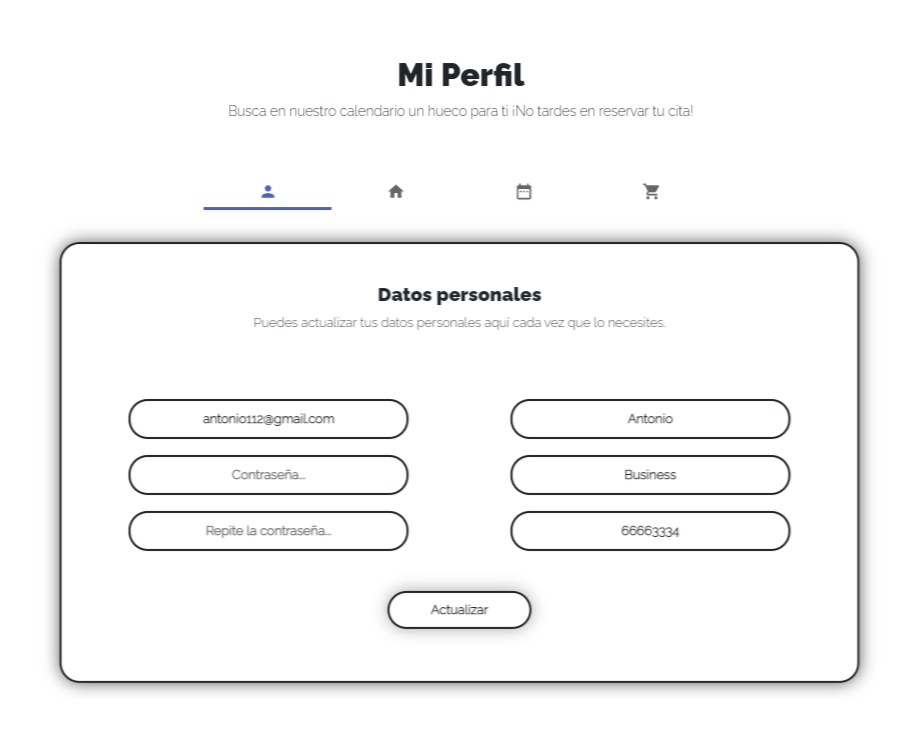
\includegraphics[scale=0.4]{images/front-end-profile-1.png}
  \caption{Página de Perfil: datos personales}
  \label{}
\end{figure}

\begin{figure}[H]
  \centering
  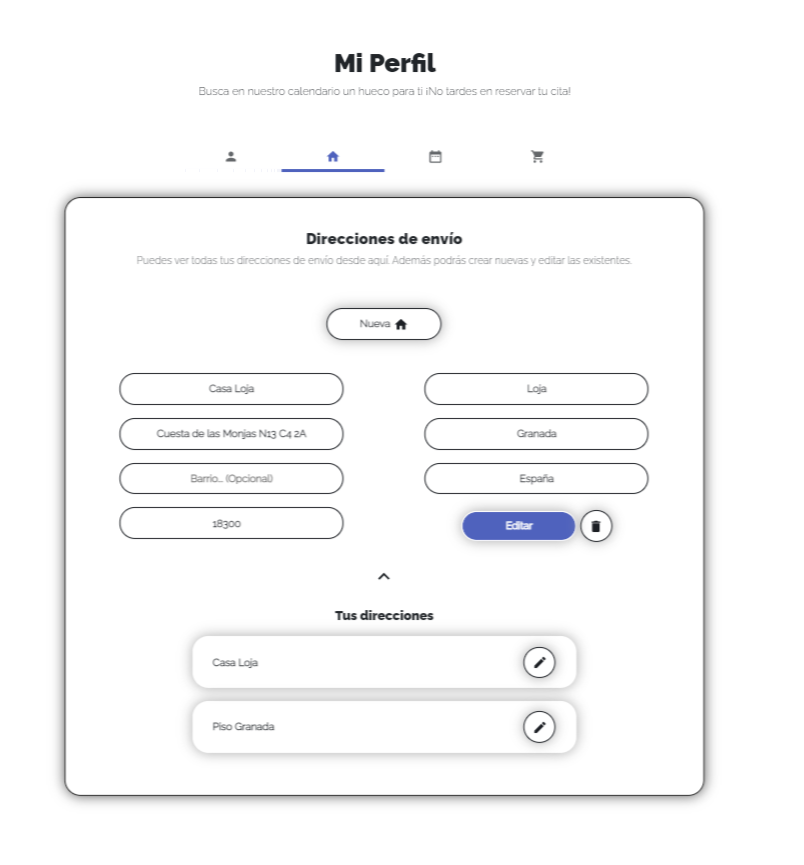
\includegraphics[scale=0.4]{images/front-end-profile-2.png}
  \caption{Página de Perfil: direcciones postales}
  \label{}
\end{figure}

\begin{figure}[H]
  \centering
  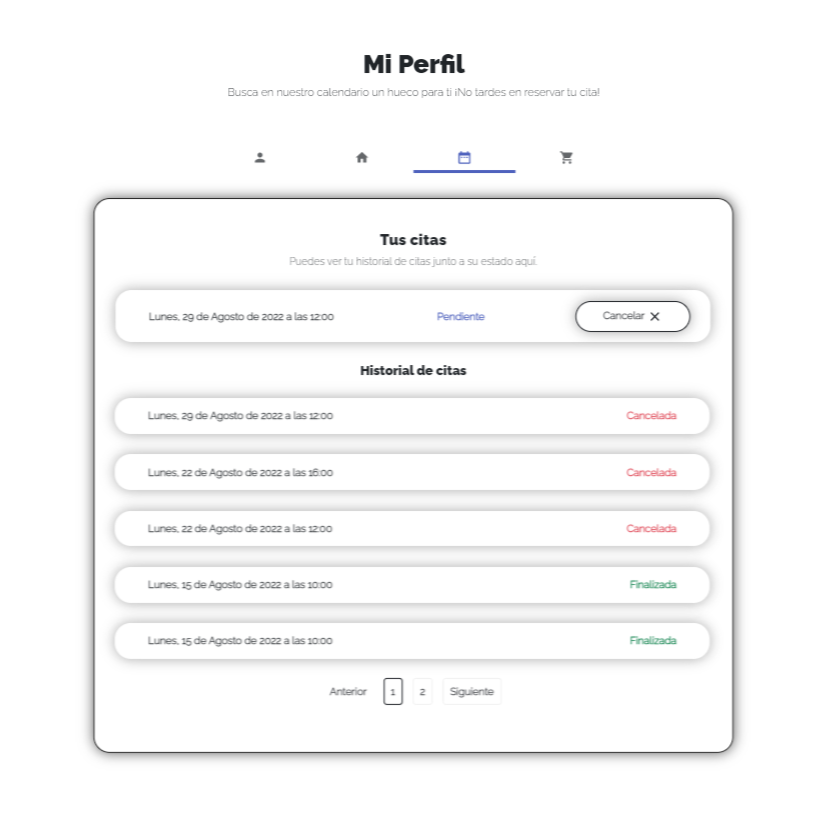
\includegraphics[scale=0.4]{images/front-end-profile-3.png}
  \caption{Página de Perfil: historial de citas}
  \label{}
\end{figure}

\begin{figure}[H]
  \centering
  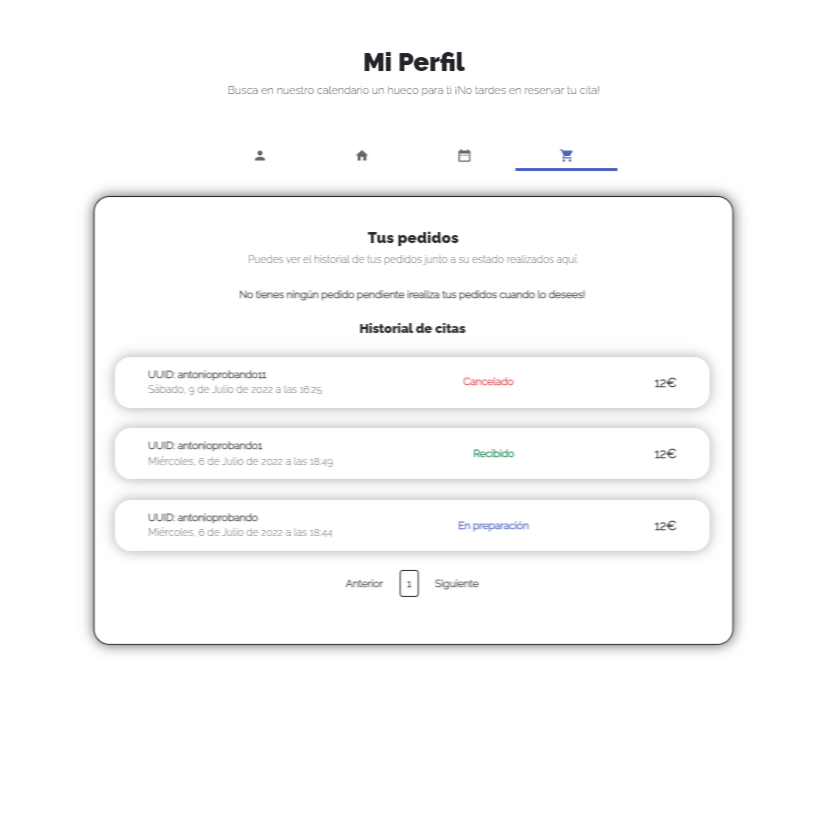
\includegraphics[scale=0.4]{images/front-end-profile-4.png}
  \caption{Página de Perfil: historial de pedidos}
  \label{}
\end{figure}